\section{API}
The API documentation explains the following classes in detail.
\subsection{Classes}
\begin{figure}[hb]
    \centering
    \fbox{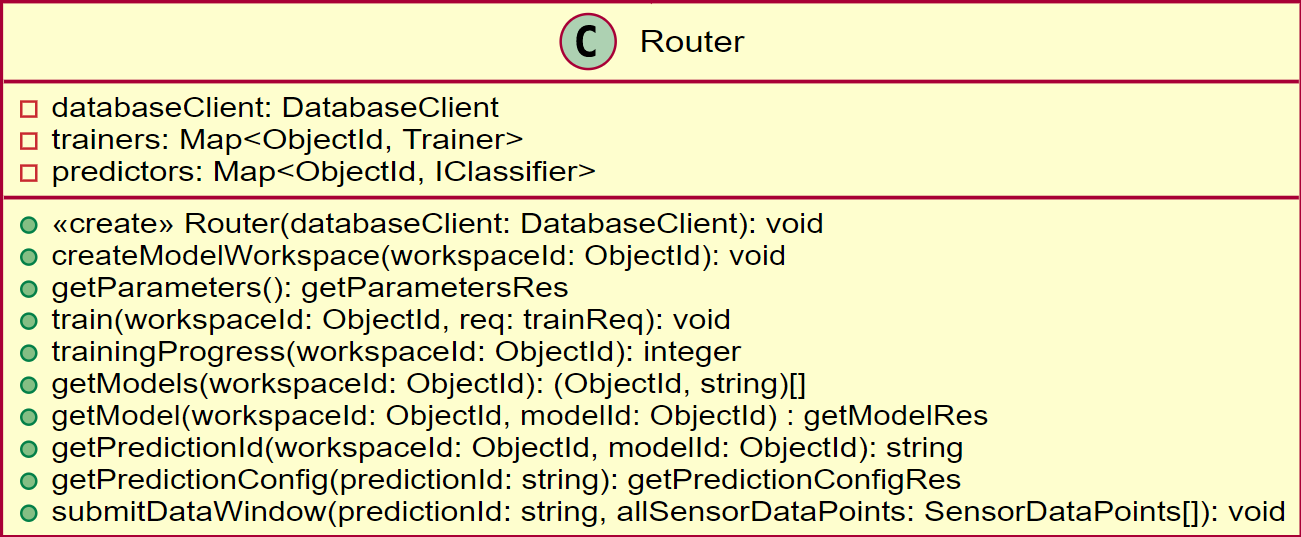
\includegraphics[width = .98\textwidth]{classes/api/router.png}}
    \caption{Router}
    \label{fig:router-class}
\end{figure}
~\\
~\\
\begin{figure}[!htb]
    \centering
    \fbox{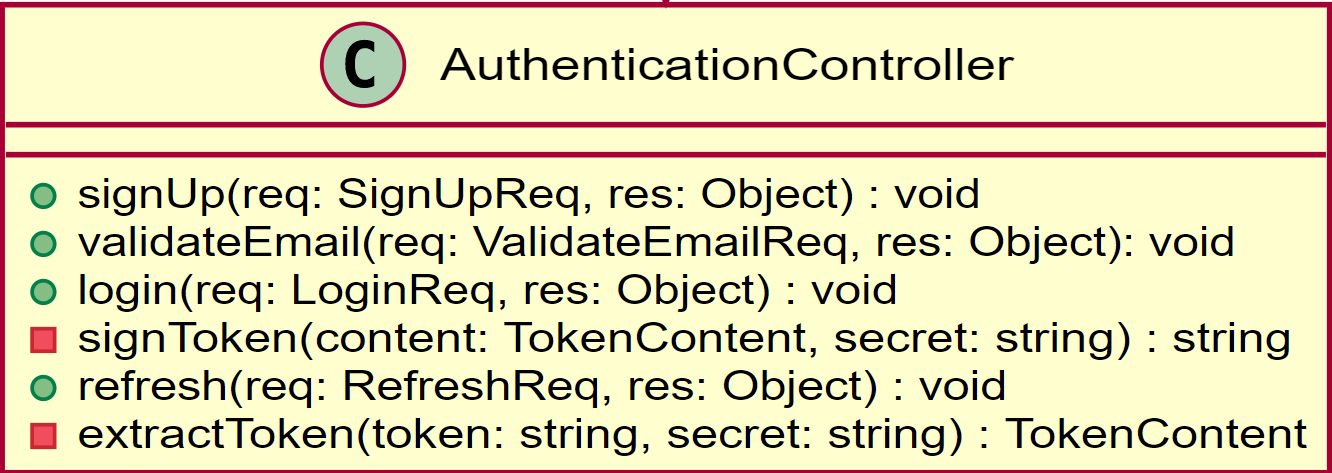
\includegraphics[width = .98\textwidth]{classes/api/auth-controller.png}}
    \caption{Authentication Controller}
    \label{fig:auth-controller}
\end{figure}
\newpage
\begin{figure}[!htb]
    \centering
    \fbox{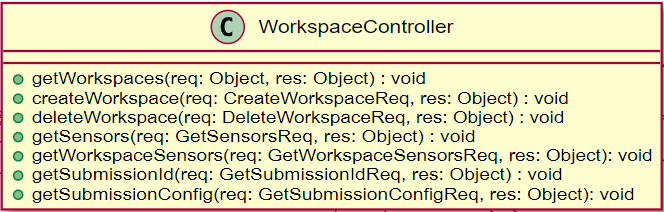
\includegraphics[width = .98\textwidth]{classes/api/workspace-controller.png}}
    \caption{Workspace Controller}
    \label{fig:workspace-controller}
\end{figure}
~\\
\begin{figure}[!htb]
    \centering
    \fbox{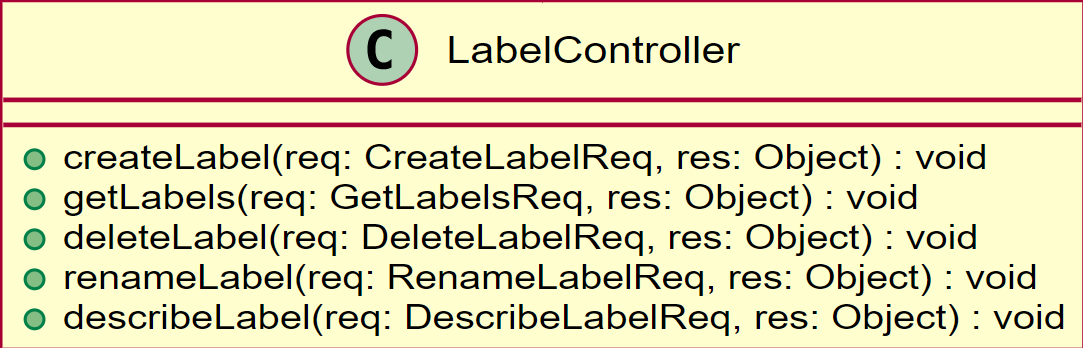
\includegraphics[width = .98\textwidth]{classes/api/label-controller.png}}
    \caption{Label Controller}
    \label{fig:label-controller}
\end{figure}
~\\
\begin{figure}[!htb]
    \centering
    \fbox{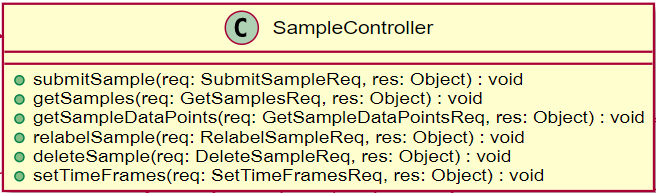
\includegraphics[width = .98\textwidth]{classes/api/sample-controller.png}}
    \caption{Sample Controller}
    \label{fig:sample-controller}
\end{figure}
%
\includepdf[pages=1,pagecommand=\subsection{Documentation}]{figures/api.pdf}
%
\includepdf[pages=2-,pagecommand={}]{figures/api.pdf}